\documentclass{beamer}
\usetheme{Warsaw}
\usepackage[T1]{fontenc}
\usepackage[right]{eurosym}
\usepackage{latexsym}
\usepackage{pgf,pgfarrows,pgfnodes,pgfautomata,pgfheaps}
\usepackage{color}
\usepackage{bbm}
\usepackage[english]{babel}
\usepackage[utf8]{inputenc}
% \usepackage[vmargin=25mm, top=20mm, bottom=25mm, left=28mm, right=28mm, includehead]{geometry}
% \usepackage{parskip}
\usepackage{csquotes}
\usepackage{german}
\usepackage{ngerman}
\usepackage{microtype}
\usepackage{amsfonts}
\usepackage{amssymb}
\usepackage{amsmath}
\usepackage{graphicx}
\usepackage{extarrows}
\usepackage{amsthm}
\usepackage{bookmark}
\usepackage{mathrsfs}
\usepackage{scrextend}
\usepackage{tikz}
\usepackage{subcaption}
\usepackage{float}
\usepackage{mathtools}
\usepackage{wrapfig}
\usepackage[singlelinecheck=false,justification=justified]{caption}
\usepackage[ruled,vlined]{algorithm2e}
\usepackage{algpseudocode}
\usepackage{mathtools}
\usepackage{hyperref}
\usepackage{graphicx}
% \usepackage{times}
\usepackage{mathptmx}
\usepackage{calrsfs}

\DeclareMathAlphabet{\pazocal}{OMS}{zplm}{m}{n}
\newcommand{\La}{\mathcal{L}}
\newcommand{\Lb}{\pazocal{L}}
\graphicspath{{./graphics/}}

\usepackage[
    left = \flqq{},%
    right = \frqq{},%
    leftsub = \flq{},%
    rightsub = \frq{} %
]{dirtytalk}


\bibliographystyle{acm}

\newcommand{\uz}{\wegde}
\newcommand{\oz}{\vee}
\newcommand*\xor{\mathbin{\oplus}}
\everymath{\displaystyle}
\newcommand{\N}{\mathbb{N}}
\newcommand{\Prob}{\mathbb{P}}
\newcommand{\Z}{\mathbb{Z}}
\newcommand{\R}{\mathbb{R}}
\newcommand{\Q}{\mathbb{Q}}
\newcommand{\C}{\mathbb{C}}
\newcommand{\E}{\mathbb{E}}
\newcommand{\source}[1]{\caption*{Source: {#1}} }
\captionsetup[figure]{font=footnotesize}
\usepackage{commath}
\usepackage{esdiff}
\DeclareMathOperator{\Var}{\mathbf{Var}}
\DeclareMathOperator{\EW}{\mathbf{E}}
\DeclareMathOperator{\WS}{\mathbf{P}}
\DeclareMathOperator{\Cov}{\mathbf{Cov}}
\newcommand{\notimplies}{\;\not\!\!\!\implies}
% Set up

\mode<presentatio>
{
  \usetheme{Frankfurt}
  \setbeamercovered{transparent}
}
\setbeamersize{text margin right = 15mm, text margin left= 15mm}
% Oder was auch immer. Zu beachten ist, das Font und Encoding passen
% m�ssen. Falls T1 nicht funktioniert, kann man versuchen, die Zeile
% mit fontenc zu l�schen.

\title[]{TC-VAE: Uncovering Out of distribution generative factors}
\author{Andreas Loehr}
\institute{Goethe Universität Frankfurt a.M.}
\date{
  \vspace{0.2cm}
  Seminar Pattern Analysis and Machine Intelligence
  \vspace{0.4cm}
  \newline 06/22/2023\\
  \vspace{0.3cm} % 0.4cm
  }
\subject{Informatik}

\let\definition\relax
\let\theorem\relax
%\let\footnoterule\relax
% \let\theorem\relax
\theoremstyle{definition}
\newtheorem{definition}[section]{Definition}
\newtheorem{intuition}{Intuition}
% \newtheorem{definition_theorem}[definition]{Definition und Satz}

\newtheorem{cus_theorem}[section]{Satz}
%\newtheorem{def_theorem}[section]{Definition und Satz}
% \newtheorem{lemma}[definition]{Lemma}
% \newtheorem{remark}[definition]{Bemerkung}
% \newtheorem{remark_ex}[definition]{Beispiel}
% \newtheorem{notation}[definition]{Notation}
\newtheorem{remark}{Bemerkung}
\begin{document}
  \AtBeginSection[]
  {
      \begin{frame}
          \tableofcontents[currentsection]
      \end{frame}
    }
    % title page
  \begin{frame}
    \begin{titlepage}
    \end{titlepage}
  \end{frame}

  %intro to generative modelling. The problem statement
  \section{Representation Learning and Generative Modeling}
    \begin{frame}
      \frametitle{The Problem statement}
      \begin{itemize}
        \item \textbf{Problem}: Given data $X \in \mathbb{R}^{d}$ find a \textit{good} latent representation $Z \in \mathbb{R}^{m}$, $d, m \in \mathbb{N}$
        \item \textbf{Example}: $X$ images of colored 3D objects, $Z$ latent representation representing shape, texture, color etc.
      \end{itemize}
     \end{frame}

     \begin{frame}
      \frametitle{Example: 3D-shapes dataset}
      \begin{figure}
        \centering
        \includegraphics[scale=0.15]{3d_shapes.png}
        \captionsetup{justification=centering}
        \caption*{\tiny{Source: https://github.com/deepmind/3d-shapes/tree/master}}
      \end{figure}
      %\vspace{-0.8 cm}
      \begin{itemize}
        \item Generative Factors $=\{[floor, wall, object] color, scale, shape, orientation\}$
      \end{itemize}
     \end{frame}

      \begin{frame}
        \frametitle{Definitions and Notation (1)}
        \begin{itemize}
          \item \textbf{Data Generative Factors:} True underlying factors / attributes of the data or generation process
          \item \textbf{OOD Data Generative Factors:} Generative Factors without variability in dataset
          % explain: no variation of this factor in entire dataset, e.g. all objects are located in center of image for OOD factor camera perspective
          \item \textbf{Latent Representation:} A vector of latent variables
        \end{itemize}
      \end{frame}

      \begin{frame}
        \frametitle{Distentanglement}
        \begin{itemize}
          \item no precise definition for disentanglement
        \end{itemize}
        \begin{definition}[Bengio et al 2013]
          A latent respresentation is called \textit{disentangled} if for each latent variable, the change in 1 generative factor leads to a change in 1 latent variable.
        \end{definition}
      \end{frame}

    \begin{frame}
      \frametitle{What makes a good latent representation?}
      \begin{itemize}
        %\item captures true generative factors of the dataset
        %\item interpretable $\rightarrow$ Optimally, \enquote{bijection} between data generative factors $\leftrightarrow$ latent representation
        % ----------------------------------------
        % complete representations are interpretable and capture true generative factors by definition
        % the lower the better
        \item complete $\rightarrow$ low (Avg.) number of latent variables required to capture a single generative factor
        % good informativeness implies balanced representation
        \item informative $\rightarrow$ Each latent variable captures a single generative factor
        %\item balanced $\to$ no single factor outweighs other factor in terms of informativeness
        \item regular $\rightarrow$ learned distribution (density) is smooth, with support having few connected components
        %, i.e. generative factors underrepresented in training data still have correspoding latent factor factors underrepresented in training data still have correspoding latent factor factors underrepresented in training data still have correspoding latent factor
        % in the sense that even generative factors which are underrepresented in the dataset do have a correspoding latent factor
      \end{itemize}
    \end{frame}

    \begin{frame}
        \frametitle{Why bother to learn good representations?}
        \begin{itemize}
          \item Facilitate downstream tasks like classification
          \item Controllable Generative modeling: control generative factors explictly by tweaking the corresponding latent variables
          % TODO: add more reasons and illustrate
        \end{itemize}
      \end{frame}

    \section{(Variational) Autoencoders}
    \begin{frame}
      \frametitle{Means to learn latent representations}
      \begin{itemize}
        \item Principal component analysis (PCA)? $\rightarrow$ Lack of interpretability
        \item (Regular) Autoencoders? $\rightarrow$ Lack of regularity
        % explain regularity - refer to Medium article/ paper
        % https://towardsdatascience.com/understanding-variational-autoencoders-vaes-f70510919f73
        \item Variational Autoencoders (VAE) $\rightarrow$ Lack of disentanglement and/ or regularity
      \end{itemize}
    \end{frame}
    % Note: Now work towards the principal contribution of the paper

    \begin{frame}
      \frametitle{Autoencoders}
      % source autoencoder illustration
      %https://miro.medium.com/v2/resize:fit:4266/1*QEmCZtruuWwtEOUzew2D4A.png
      %\begin{center}
      \begin{figure}
        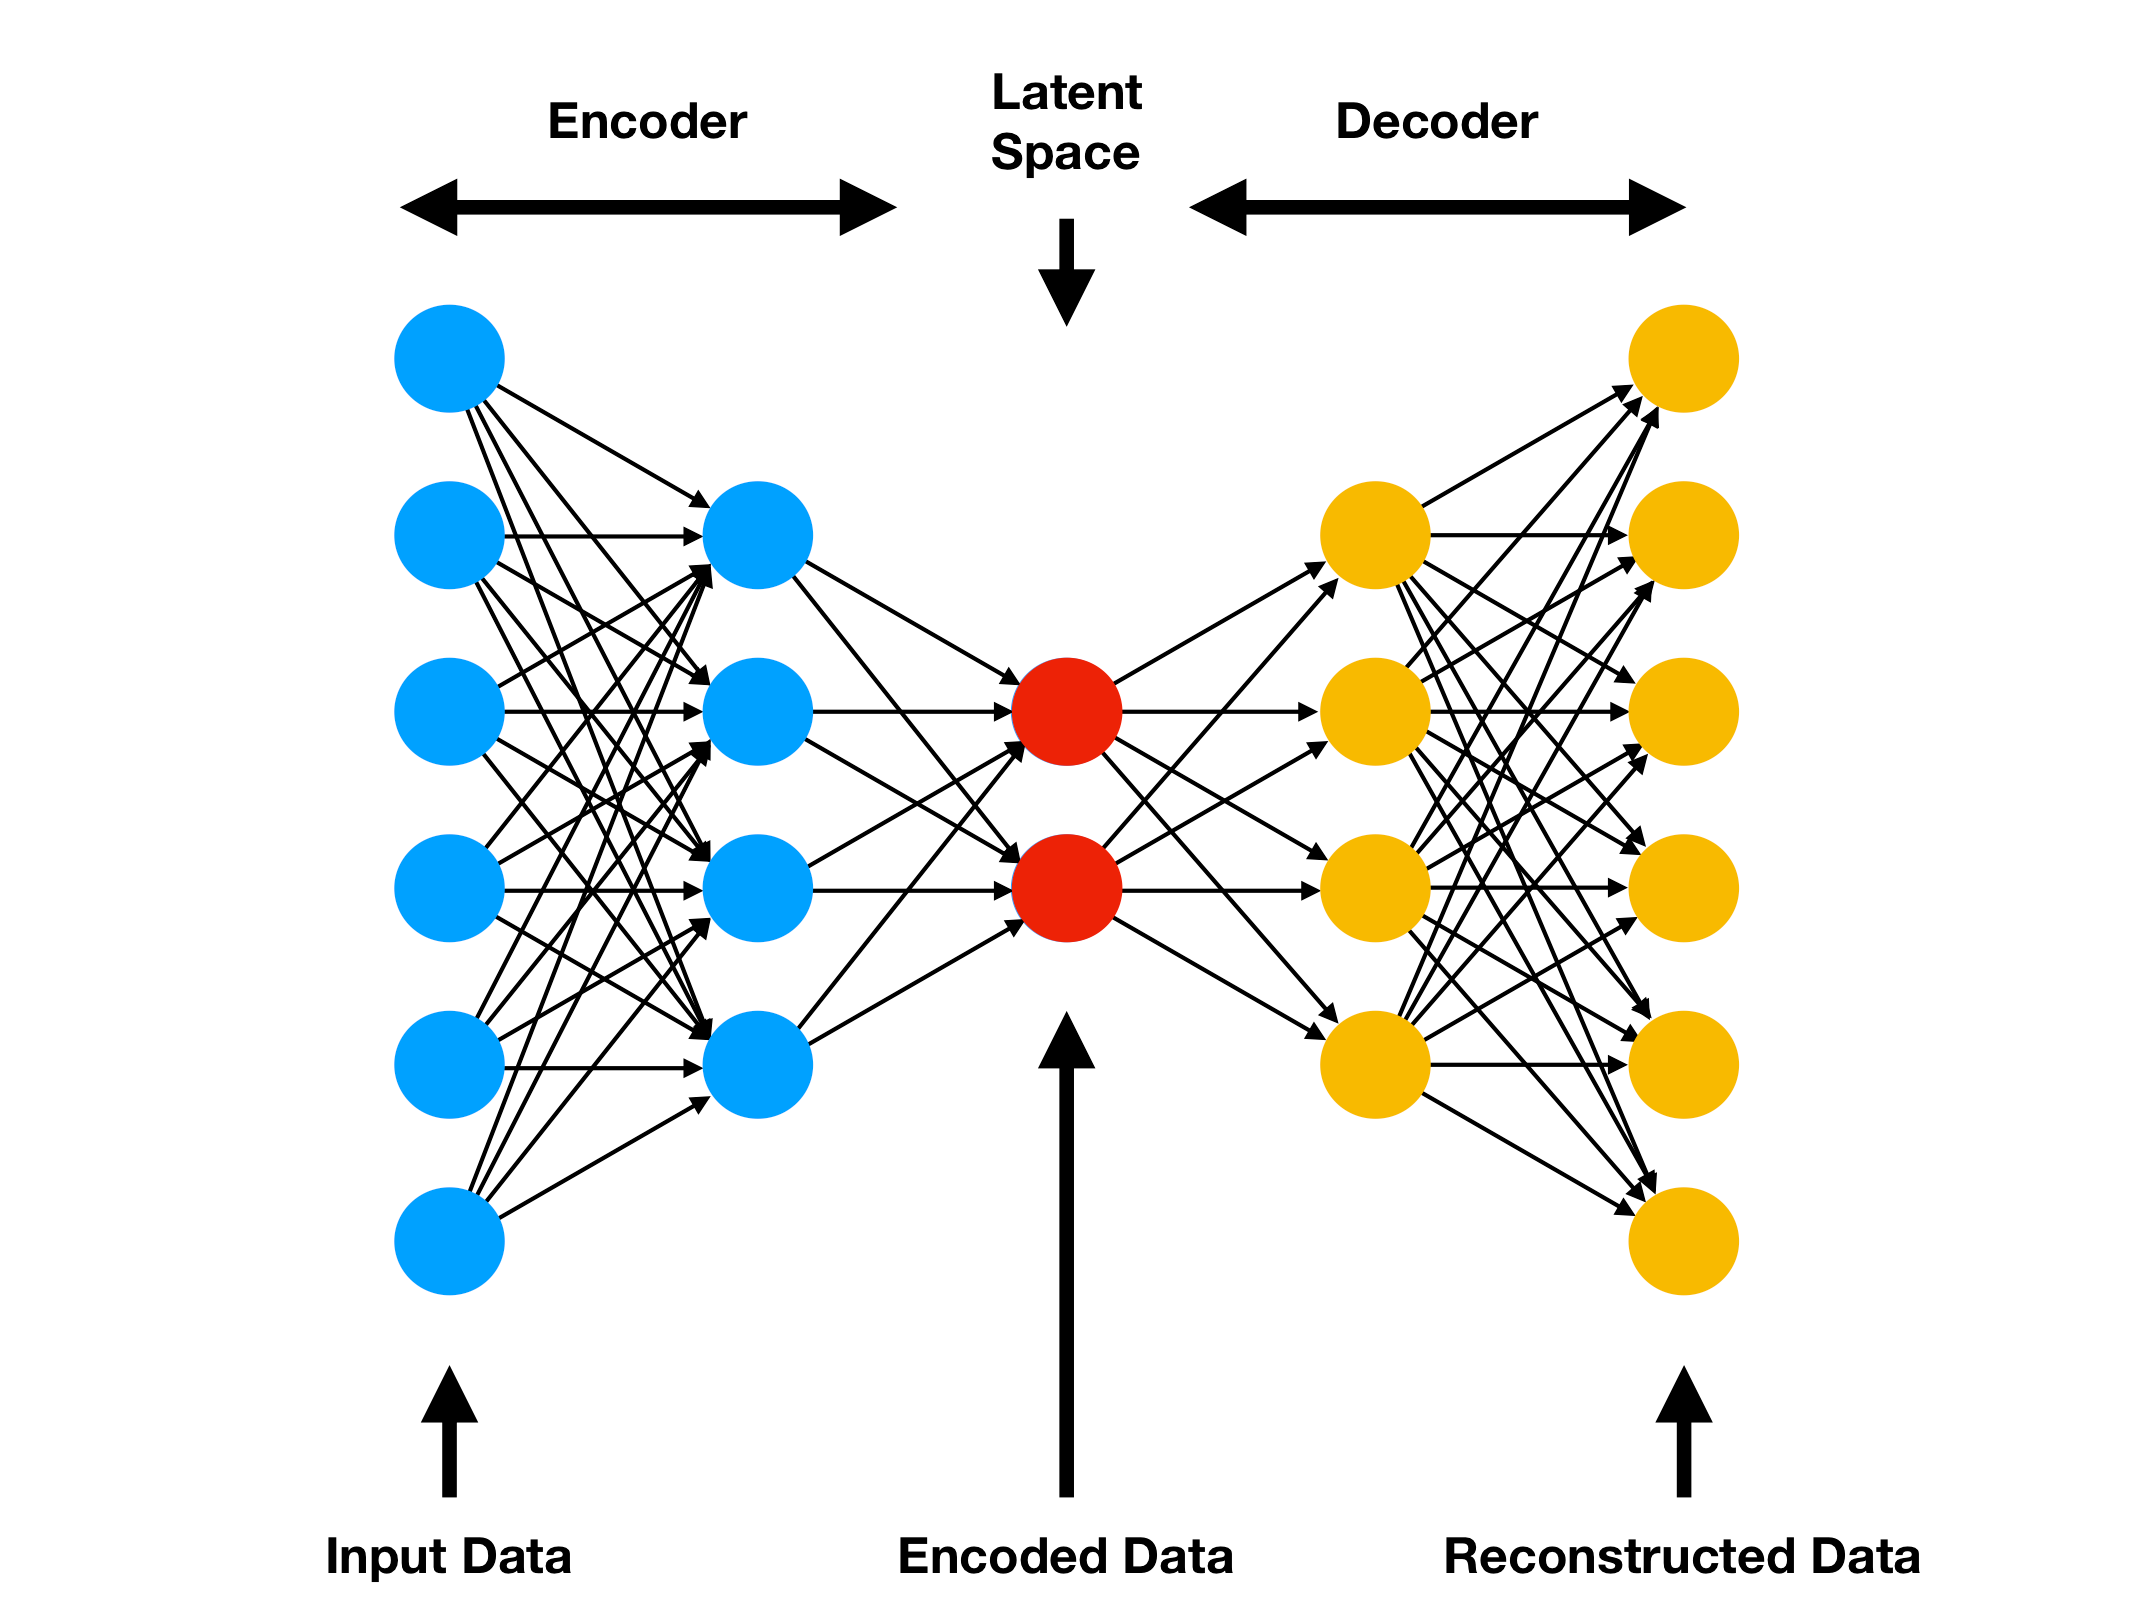
\includegraphics[scale= 0.1]{Autoencoder_illustration.png}
        \captionsetup{justification=centering}
        \caption*{\tiny{Source: https://medium.com/autoencoder-for-anomaly-detection/autoencoder-for-anomaly-detection-db6178ad07b2}}
        % explain graphics quickly
      \end{figure}
      % \end{center}

    \end{frame}
    \begin{frame}
      \frametitle{Variational Autoencoders}
      \begin{figure}
        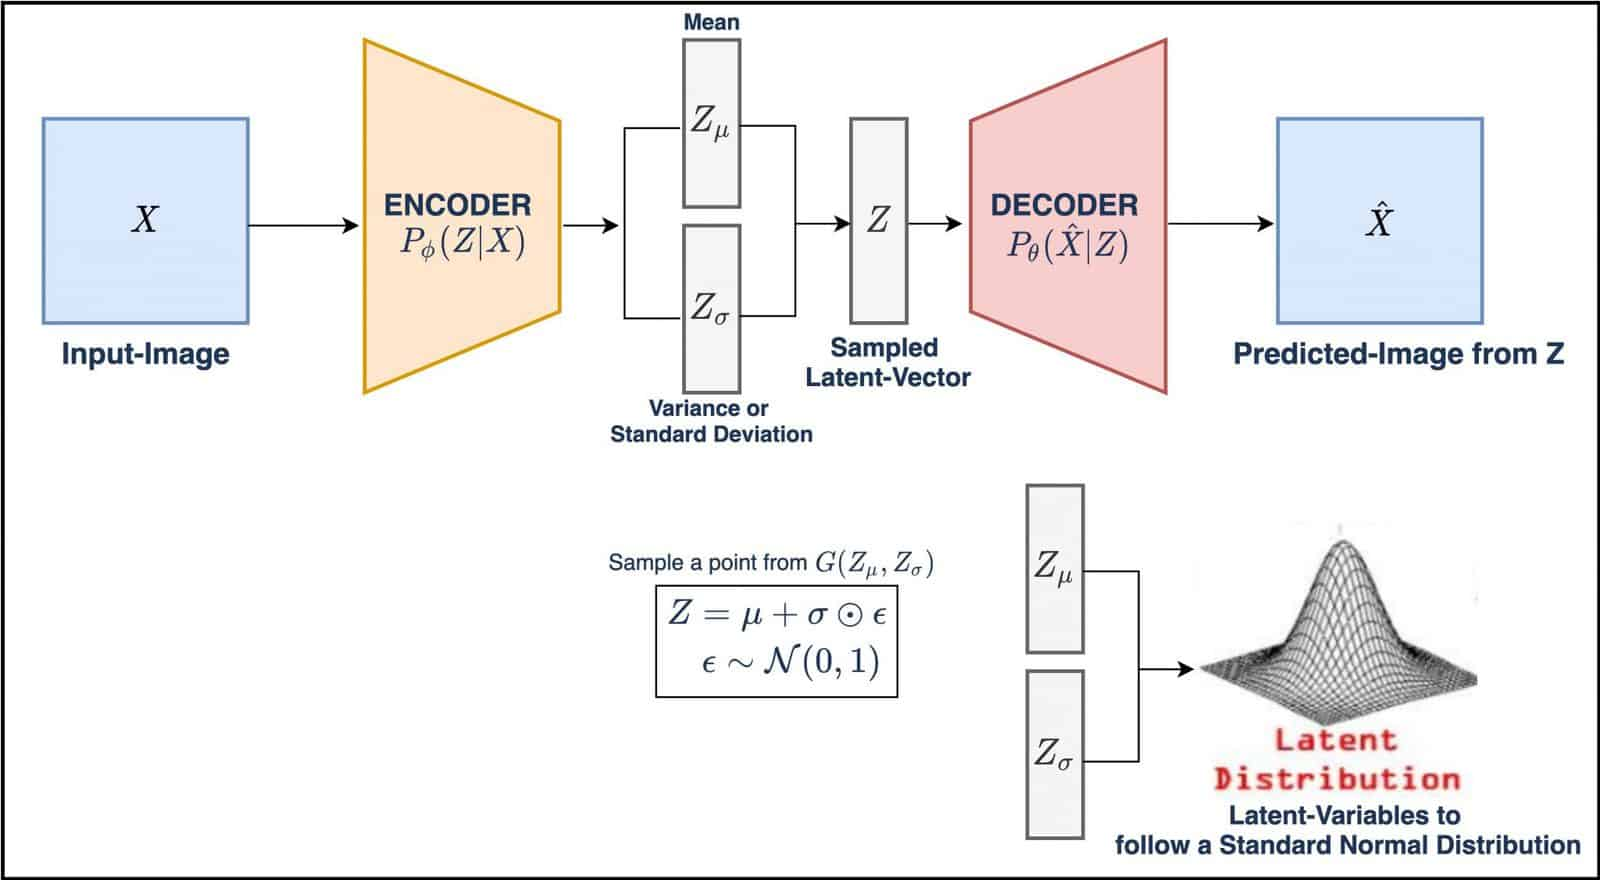
\includegraphics[scale=.125]{vae-diagram.jpg}
        \captionsetup{justification=centering}
        \caption*{\tiny{Source: https://learnopencv.com/variational-autoencoder-in-tensorflow}}
      \end{figure}
      \vspace{-5mm}
      \begin{itemize}
        \item Generative model consisting of probabilisitic encoder and decoder
        \item (Neural Network) encoder \& decoder parametrize conditional probability distributions over latent space and data respectively
      \end{itemize}
      % explain the graphics

    \end{frame}
    \begin{frame}
      \frametitle{Training Variational Autoencoders (1)}

      \begin{itemize}
        \item (Original) objective: maximizing likelihood of data, i.e. find $\theta$ s.t. $p_{\theta}(X) \approx p(X)$
        % introduce latent variables since latent variable models are powerful in that they are capable of learning really complex probabililty distributions
        \item Due to latent variables, optimization is intractible $\rightarrow$ approximate $p_{\theta}(Z \mid X)$ and make tractable
        \item Approximate inference using parametrized model $q_{\phi}(Z \mid X)$ % to approximate $p_{\theta}(Z \mid X)$
        \item Actual objective: \textbf{Variational lower bound (ELBO)} $\rightarrow$ serves as lower bound to the likelihood of observed data
      % TODO: VAE objective insert and explain
     \end{itemize}
    \end{frame}

    \begin{frame}
      \frametitle{Kullback-Leibler Divergence}
      Let $p(x), q(x)$ be 2 (univariate) probability densities.
      \begin{definition}[Kullback-Leibler Divergence ($D_{KL}$)]
       $D_{KL}(p \Vert q = \int p(x) \log \frac{p(x)}{q(x)} dx$
      \end{definition}
      \begin{intuition}
        Measures the similarity betweeen 2 probability distributions.
      \end{intuition}

    \end{frame}
    \begin{frame}
      \frametitle{Training Variational Autoencoders (2)}
      The ELBO is given as
      \begin{align*}
        \Lb_{\phi, \theta}(X) = \E_{q_{\phi}(Z \mid X)}[\log p_{\theta}(X, Z) - \log q_{\phi}(Z \mid X)].
      \end{align*}
      Maximiziation of the ELBO results in
      \begin{itemize}
        \item minimization of $D_{KL}(q_{\phi}(Z \mid X) \Vert p_{\theta}(Z \mid X))$
             \item maximation of $\log p_{\theta}(X)$
      \end{itemize}
    \end{frame}

    \begin{frame}
      \frametitle{Shortcomings}
      \begin{itemize}
        \item \enquote{low dimensional} latent space $\to$ blurry reconstructions (lack of information in latents)
        \item \enquote{high dimensional} latent space $\to$ low degree of distentanglement and no regularity
        % TODO: Learned distribution in high dimensional space has disperded support -> no regularity
      \end{itemize}
    \end{frame}

    \begin{frame}
      \frametitle{Trying to Fix VAEs}
      \begin{itemize}
        \item change of optimization objective to encourage desired behavior
        \item All about trade-off between reconstruction and disentaglement
        \item Important condition on new objectives: Lower bound to log likelihood of data
        \begin{enumerate}
          \item $\beta$-VAE ($\beta > $ 1): Poor reconstruction (information retained in latent rep. not sufficient)
          \item Factor VAE:
          \item ...
        \end{enumerate}
      \end{itemize}
    \end{frame}


    \section{TC-VAEs}
    \begin{frame}
      \frametitle{Prerequisites}
      \begin{itemize}
        \item $X = (X_{1}, \dots, X_{d})$ random variable (rv) w/ density $p(x)$ and distribution $P^{X}$.
        \item $Z = (Z_{1}, \dots, Z_{m})$ rv w/ density $p(z)$ and distribution $P^{Z}$.
        \item In the following we use $p(x)$ and $P^{X}$  interchangeably.
              \item Following definitions have conditional counterparts
      \end{itemize}
    \end{frame}

    \begin{frame}
      \frametitle{Shannon Entropy}
      \begin{definition}[Shannon Entropy]
        $H(X) \coloneqq -\mathbb{E}_{P^{X}}[\log p(x)] = -\int_{\R^{d}}p(x) \log p(x) dx$
      \end{definition}
      % Note: def for rv continous, in discrete case, replace Rd by N and dx by counting measure
      % Note: def is equivalent for conditional distributions
      \begin{intuition}
       Measures the randomness of a random variable.
     \end{intuition}
     \begin{example}
       \begin{itemize}
         \item Dirac Measure in a point $\rightarrow H(X) = 0$
               \item Coin Flip $\rightarrow H(X) = 1$
       \end{itemize}
     \end{example}
    \end{frame}

    \begin{frame}
      \frametitle{Mutual Information}
      \begin{definition}[Mutual Information]
        $I(X, Z) \coloneqq H(X) + H(Z) - H(X, Z) = H(Z) - H(Z \mid X)$
      \end{definition}
      % Note: def for rv continous, in discrete case, replace Rd by N and dx by counting measure
      \begin{intuition}
        Reduction in uncertainty of one rv given another rv.
        % Or what is left actually. Understand this
      \end{intuition}
    \end{frame}

    \begin{frame}
      \frametitle{Total Correlation}
      \begin{definition}[Total Correlation (TC)]
        $TC(X) \coloneqq D_{KL}\left[P^{X} \large  \Vert \prod_{i=1}^{d}P^{{X_{i}}}\right] $
      \end{definition}
      \begin{intuition}
        TC measures the amount of information \textit{shared} among the random variables.
        % point out why using the definition
      \end{intuition}
    \end{frame}

    \begin{frame}
      \frametitle{Total Correlation as an objective (1)}
      New objective given by
      \begin{align*}
        \underset{\theta}{\arg \max}TC_{\theta}(Z, X) \coloneqq TC_{\theta}(Z) - TC_{\theta}(Z \mid X).
      \end{align*}
      \begin{intuition}
        Equivalent to minimizing 2nd term $\iff$ given $X$, information shared among components of $Z$ is reduced.
        \newline
        More intuition if viewed in information theoretic framework.
      \end{intuition}
    \end{frame}
    % Why this objective? More insight from information theoretic pov

    \begin{frame}
      \frametitle{Total Correlation as an objective (2)}
      Rewrite TC in terms of MI:
      \begin{align*}
        TC_{\theta}(Z, X) = \left(\sum_{k=1}^{m}I_{\theta}(Z_{k}, X)\right) - I_{\theta}(Z, X)
      \end{align*}
      \begin{intuition}
        \begin{itemize}
          \item Maximizing each terms $I(Z_{k}, X)$ $\to$ promotes single latent variable to \enquote{share} information with $X$
          \item Minimizing $I(Z, X)$ promotes independence of $Z$ conditional on $X$ (VIB term)
          % see this by writing I(Z, X) = I(X) - I(X | Z) = I(Z) - I(Z | X) which is minimized if Z is independent condiitonal on X
        \end{itemize}
      \end{intuition}
    \end{frame}

    \begin{frame}
      \frametitle{Total Correlation as an objective (3)}
      TODO: Make sure CMI known, defined
      Writing TC in terms of CMI:
      \begin{align*}
        TC_{\theta}(Z, X) = \frac{1}{m}\sum_{k = 1}^{m}\left[ (K-1) I_{\theta}(Z_{k}, X) - I_{\theta}(Z_{\neq k}, X \mid Z_{k})\right]
      \end{align*}
      \begin{intuition}
       \begin{itemize}
         \item Maximizing each terms $I(Z_{k}, X)$ $\to$ promotes single latent variable to \enquote{share} information with $X$
         \item Minimizing $I_{\theta}(Z_{\neq k}, X \mid Z_{k})$ promotes balance of information related to each single latent variable (CEB term)
       \end{itemize}
      \end{intuition}
    \end{frame}

    \begin{frame}
      \frametitle{A convex lower bound of TC objective}
      \textbf{Problem}: Intractable optimization problem.
\newline
      \vspace{.5 cm}
      $\to$ need lower bound to maximize.
      \newline
      Convex Combination of different representation of TC
      \begin{center}
        $\underset{\text{derivation}}{\leadsto}$
      \end{center}
      \begin{align*}
        \begin{split}
          &TC_{\theta}(Z, X) \geq \E_{q_{\theta}(Z \mid X)}[\log p_{\phi}(X \mid Z)]\\
          &- \frac{\alpha}{M-\alpha} \sum_{k=1}^{m}D_{KL}(q_{\theta}(Z_{k} \mid X) \Vert r_{p}(Z_{p} \mid X))\\
          &- \frac{1-\alpha}{1 - \frac{\alpha}{m}}D_{KL}(q_{\theta}(Z \mid X) \Vert r(Z)).
        \end{split}
      \end{align*}
    \end{frame}
    \begin{frame}
      \frametitle{A convex lower bound of TC objective (details)}
      \begin{itemize}
              \item $\alpha$ Hyperparamter from convex combination balancing effects of VIB and CMI terms
        \item $r(Z) = \mathcal{N}(0, \mathbf{I})$
        \item $r_{p}(Z_{p} \mid X) = \mathcal{N}(\mu_{p}, \sigma_{p})$
        \item $\mu_{p} \coloneqq \frac{\sum_{k=1}^{m}\frac{\mu_{k}}{\sigma_{k}^{2}}}{\sum_{k=1}^{m}\frac{1}{\sigma_{k}^{2}}}$
        \item $\sigma_{p}^{2} \coloneqq \frac{1}{\sum_{k=1}^{m}\frac{1}{\sigma_{k}^{2}}}$
              \item $\mu_{k}, \sigma_{k}$ are outputs from encoder network.
      \end{itemize}
    \end{frame}



  \section{Experiments and Results}
    \begin{frame}
      \frametitle{Experiment Design}
      \begin{itemize}
        \item \textbf{Baseline Models}: $\beta$-VAE, Factor VAE with similar Encoder and Decoder Models
        \item \textbf{Datasets}: 3D shapes dataset and unbalanced 3D shapes dataset, $\dots$
        %% explain U3D shapes dataset, stress that there are more datasets used in comparison than those listed
        \item \textbf{Evaluation Methods}:
          \begin{enumerate}
            \item Qualitative: Latent space traversals
            % Explain latent space traversals
            \item Quantitative: DCI, WSEPIN measuring Disentanglement, Completeness and Informativeness
            % Explain DCI, WSPEIN and study those metrics to understand their meaning
          \end{enumerate}
        \item Quantitaive Results report an average of 3 evaluations using different seeds
      \end{itemize}
    \end{frame}

    \begin{frame}
      \frametitle{Results - Qualitative (1)}
      \begin{itemize}
        \item Traversals through latent space show discovery of 2 OOD generative factors in 3D objects dataset
      \end{itemize}
      \begin{figure}
        \centering
        \includegraphics[scale=0.18]{latent_traversals_TC.png}
        \captionsetup{justification=centering}
        \caption*{\tiny{Source: original paper}}
        % images generated by varying one latent variable at a timea
      \end{figure}
      \begin{itemize}
        \item Object dim and object color are not fully disentangled
      \end{itemize}
    \end{frame}

    \begin{frame}
      \frametitle{Results - Qualitative (2)}
      \begin{itemize}
        \item OOD samples generated by TC-VAE and baseline models
      \end{itemize}
      \begin{figure}
        \centering
        \includegraphics[scale=0.13]{comp_OOD_samples.png}
        \captionsetup{justification=centering}
        \caption*{\tiny{Source: original paper}}
        % comment these findings
        % one can see that
      \end{figure}
    \end{frame}

    \begin{frame}
      \frametitle{Results - Quantitative (1)}
      Results on \textbf{balanced} datasets:
      \begin{figure}
        \centering
        \includegraphics[scale=0.18]{quantitative_balanced.png}
        \captionsetup{justification=centering}
        \caption*{\tiny{Source: original paper}}
        % images generated by varying one latent variable at a timea
      \end{figure}
      \begin{itemize}
        \item Outperforming baseline models on balanced dataset in terms of presented evaluation metrics

        \item Performance on unbalanced datasets falls short of performance of baseline models
      \end{itemize}
    \end{frame}

    \begin{frame}
      \frametitle{Results - Quantitative (2)}
      Results on \textbf{unbalanced} datasets:
      \begin{figure}
        \centering
        \includegraphics[scale=0.18]{quantitative_unbalanced.png}
        \captionsetup{justification=centering}
        \caption*{\tiny{Source: original paper}}
        % images generated by varying one latent variable at a timea
      \end{figure}
      \begin{itemize}
        \item Outperformance in terms of informativenes
        \item Stronger imbalance lead to better performance of Factor VAE
      \end{itemize}
    \textbf{BUT:} Quantiative and qualitative results do not converge $\rightarrow$ questionable results
    \end{frame}
    \section{Discussion and Conclusion}

    \begin{frame}
      \frametitle{Discussion}
      \begin{itemize}
        \item Inspiration from Multiview representation learning
        \item Uncovering OOD generative factors $\equiv$ inferring missing views
        \item Experimental validation that TC-VAE is capable of uncovering OOD generative factors (really recognizing them as generative factors instead of treating them as side effects)
        \item unbalanced generative factors in dataset $\implies$ disentanglement deteriorates.
        \item Consistent outperfomance in terms of informativeness
      \end{itemize}
    \end{frame}

    \begin{frame}
      \frametitle{Conclusion}
      \begin{itemize}
        % Main shortcoming
        \item Design of the lower bound leads to balanced representations at cost of minor shortcomings in disentanglement (probably result of trade-off induced by the different terms in lower bound)
        \item Weak performance on unbalanced datasets in terms of disentanglement
      \end{itemize}
    \end{frame}

    \begin{frame}
      \frametitle{Criticism and Comments}
      \begin{enumerate}
        \item The concept of disentanglement is not clearly defined. Sometimes its equivalent to independence, sometimes not.
        \item Datasets used are toy datasets. Effectiveness remains to be shown on real datasets
        \item Not clear which definitions of TC they are using. Although they are citing the MVRL paper quite often, the deifnition of TC does not match
      \end{enumerate}
    \end{frame}

    \begin{frame}
      \frametitle{Literature}
      Book Elements of information theory
      TODO
    \end{frame}


   \end{document}
